\chapter{Building A Vehicle Counting Application Using Density Estimation}

In this thesis, Application will build will serve for client to couting objects in order to archive that the application separate each object type then train it separately. \\ 

\textbf{Training Pharse: }


 \textbf{FOR ALL} list of object type \textbf{DO}
        \begin{enumerate}
          \item calculate features of each sample of \textbf{objectType} 
          \item calculate ground truth of each sample of \textbf{objectType} 
          \item train model for \textbf{objectType} 
        \end{enumerate}
 
Application has features:
\begin{enumerate}
  \item Get sample from video, and mark object with height and width
  \item Train model with sample create from Marker
  \item Run the estimation with model train from Trainer
\end{enumerate}
\section{Application Requirements Analysis}
Application has been divide into  3 main module
\begin{enumerate}
  \item Marker: for Get sample from video, define object types, mark instances of objects types in samples
  \item Trainer: Train model with sample create from Marker
  \item Runner: Run the estimation with model train from Trainer
\end{enumerate}
\begin{center}
  \begin{figure}[H]
    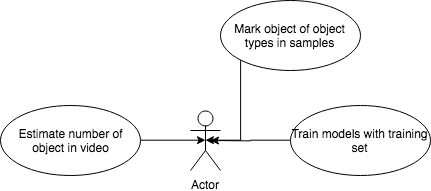
\includegraphics[width=\textwidth]{Chapters/Fig/usecase}
    \label{usecasediagram}
    \caption{Use case diagram}
  \end{figure}
\end{center}

\begin{table}[H]
\begin{center}
  \begin{tabular}{ | c | l | } 
  \hline
  \textbf{Actor} & \textbf{Use case} \\
  \hline
  \multirow{3}{4em}{Client} Mark instances of objects types in samples\\
  &Train models with samples\\
  &Run estimate with model in video\\
  \hline
  \end{tabular}
  
\end{center}
\caption{Use case table}\label{tab:usecase}
\end{table}

\section{Functional Requirements Analysis}

Table below show detail the specification for each of use cases.

\begin{table}[H]
  \begin{center}
    \begin{tabular}{ | c | l | } 
    \hline
    \textbf{Use case ID} & UC01 \\
    \hline
    \textbf{Use case name} & Mark instances of objects types in samples \\
    \hline
    \textbf{Description} & Mark instances of objects types in samples \\
    \hline
    \textbf{Actor} & Client \\
    \hline
    \textbf{Trigger} & press button add object \\
    \hline
    \textbf{Input} & object type, sample \\
    \hline
    \textbf{Output} & Show mark in viewer \\
    \hline    
    \multirow{2}{4em}{\textbf{Preconditions}} & Open the application, click on marker button\\ 
    & objects has been added, Get Sample From video, lock the object type \\
    \hline
    \multirow{2}{4em}{\textbf{Main Flow}}  & Click object type on list of object and samples on list of samples,\\
    & then click button add object, then set height, width then click done \\
    \hline
    \multirow{3}{4em}{\textbf{Alternative Flow}} & Click object type on list of object and samples on list of samples,\\
    & then click button add object, then set height, width \\
    & but have been mistake on set click clear \\
    \hline
    \textbf{Exceptions} & None \\
    \hline
    \textbf{Frequency of use} & High \\
    \hline
    \end{tabular}
  \end{center}
  \caption{Use case UC01}\label{tab:uc1}
\end{table}

\begin{table}[H]
  \begin{center}
    \begin{tabular}{ | l | l | } 
    \hline
    \textbf{Use case ID} & UC02 \\
    \hline
    \textbf{Use case name} & Train models with sample \\
    \hline
    \textbf{Description} & Train models with sample\\
    \hline
    \textbf{Actor} & Client \\
    \hline
    \textbf{Trigger} & press button start train\\
    \hline
    \textbf{Input} & Number of iter, same size gauss \\
    \hline
    \textbf{Output} & show status: Train done \\
    \hline    
    \textbf{Preconditions} & Has data from marker, Open the application \\
    \hline
    \multirow{3}{4em}{\textbf{Main Flow}}  & Click Open folder, choose folder that marker data saved\\
    & then click open dictionary file choose dictionary file in csv form,\\
    & then click start train \\
    \hline
    \multirow{3}{4em}{\textbf{Alternative Flow}} & Click Open folder, choose folder that marker data saved\\
    & then click open dictionary file choose dictionary file in csv form\\ 
    & change value of iterations, then click start train \\
    \hline
    \textbf{Exceptions} & None \\
    \hline
    \textbf{Frequency of use} & Normal \\
    \hline
    \end{tabular}
  \end{center}
  \caption{Use case UC02}\label{tab:uc2}
\end{table}


\begin{table}[H]
  \begin{center}
    \begin{tabular}{ | l | l |} 
    \hline
    \textbf{Use case ID} & UC03 \\
    \hline
    \textbf{Use case name} & Run estimate with model in video \\
    \hline
    \textbf{Description} & Run estimate with model in video\\
    \hline
    \textbf{Actor} & Client \\
    \hline
    \textbf{Trigger} & press button $>$\\
    \hline
    \textbf{Input} & avg All object types height, width, downscale, frame step  \\
    \hline
    \textbf{Output} & show estimate data, and frame process \\
    \hline    
    \textbf{Preconditions} & Has data from marker, trainer, Open the application \\
    \hline
    \multirow{3}{4em}{\textbf{Main Flow}}  & Click Open folder, choose folder that marker data saved\\
    & then click open dictionary file choose dictionary file in csv form \\
    & Click Open video file, choose video will estimate then click button $>$\\
    \hline
    \multirow{5}{4em}{\textbf{Alternative Flow}} & Click Open folder, choose folder that marker data saved\\
    & then click open dictionary file choose dictionary file in csv form \\
    & Click Open video file, choose video will estimate\\ 
    & change value of avg All object types height, width downscale, frame step\\
    & then click button $>$\\
    \hline
    \textbf{Exceptions} & None \\
    \hline
    \textbf{Frequency of use} & Normal \\
    \hline
    \end{tabular}
  \end{center}
  \caption{Use case UC07}\label{tab:uc7}
\end{table}



\section{User Interface design}

Figure below is screen design in application. Design (file .ui) has been create by QT creator

\begin{center}
  \begin{figure}[H]
      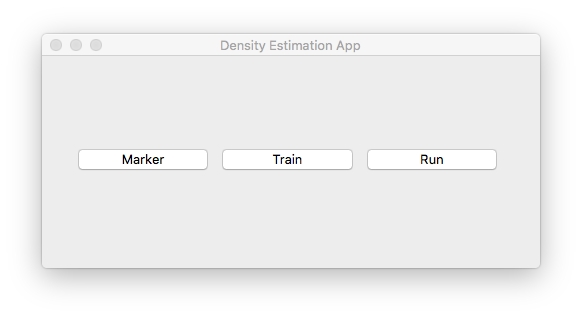
\includegraphics[width=\textwidth]{Chapters/Fig/Appllication}
      \caption{Main Application}
      \label{fig:mainapp}
    \end{figure}

  Fig \ref{fig:mainapp} show the main application, client can easily see three module \textbf{Maker, Trainer, Runner}

    \begin{figure}[H]
      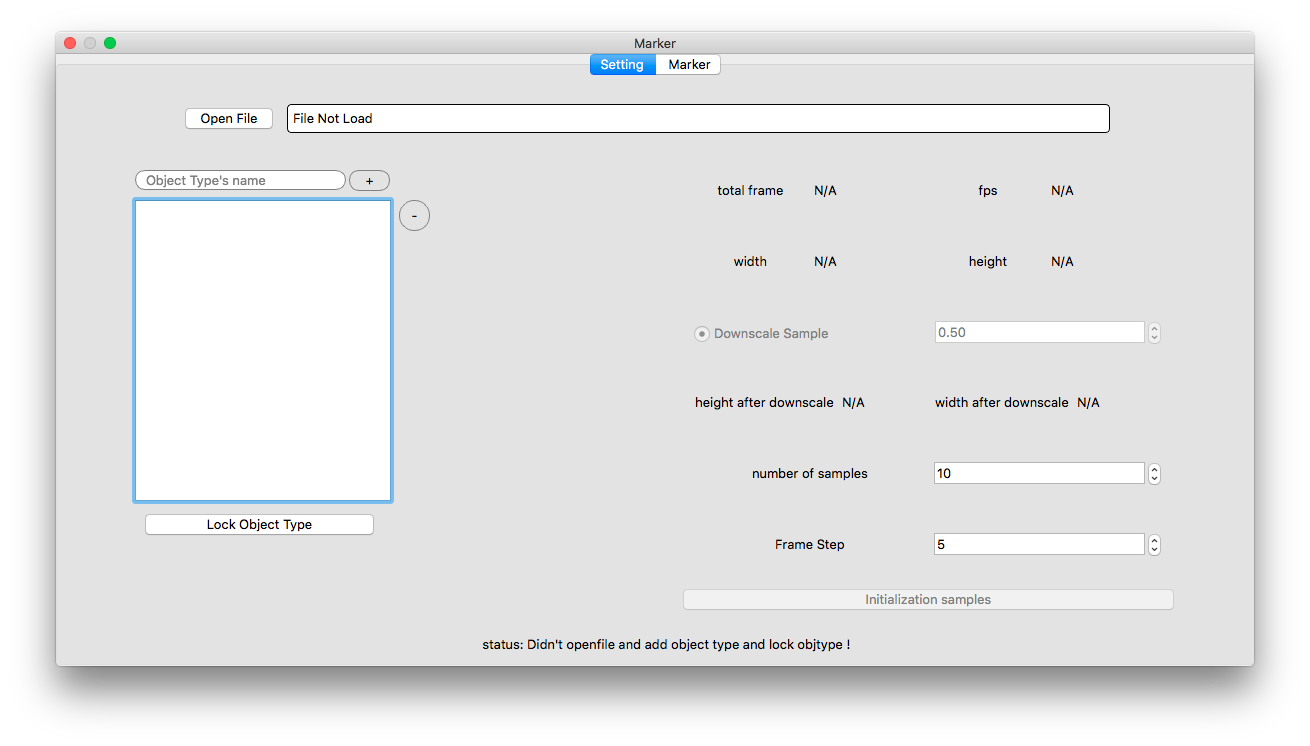
\includegraphics[width=\textwidth]{Chapters/Fig/marker-setting}
      \caption{Marker Setting Tab}
      \label{fig:marker-setting}
    \end{figure}

  Fig \ref{fig:marker-setting} show the marker setting tab, where client can change the setting and initialization before mark the object \textbf{Maker, Trainer, Runner}\\

    \begin{figure}[H]
      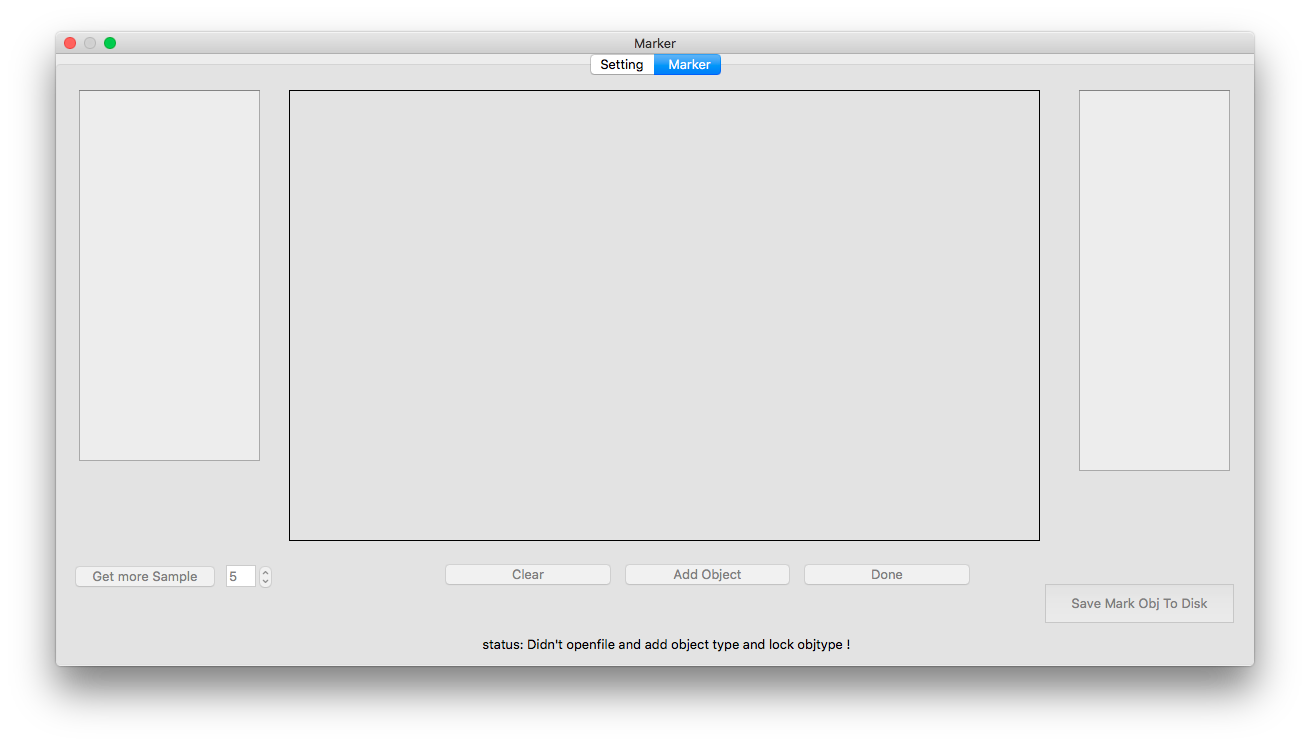
\includegraphics[width=\textwidth]{Chapters/Fig/marker-marker}
      \caption{Marker Marker Tab}
      \label{fig:marker-marker}
    \end{figure}

  Fig \ref{fig:marker-marker} show the marker marker tab, where client can mark the object. The viewer In the center of the sceen client can easily to focus on marking task. \\

    \begin{figure}[H]
      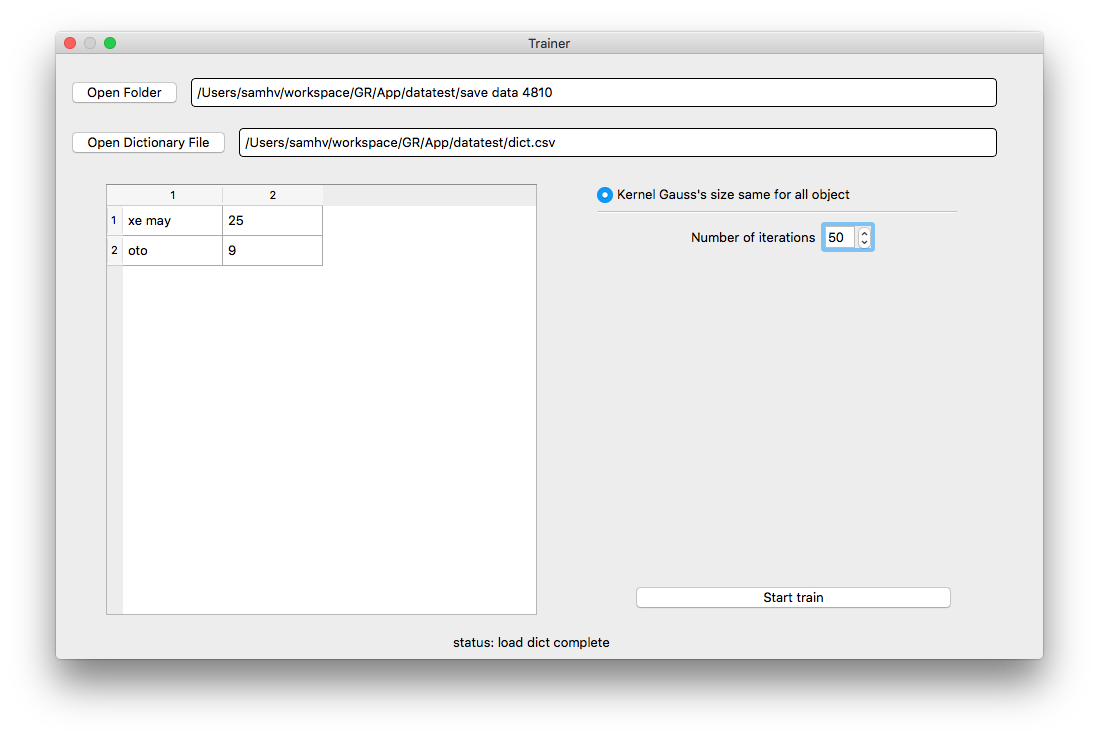
\includegraphics[width=\textwidth]{Chapters/Fig/Trainer}
      \caption{Trainer}
      \label{fig:Trainer}
    \end{figure}

  Fig \ref{fig:Trainer} show the trainer, where client load the samples and dictionary train the model.\\
 
    \begin{figure}[H]
      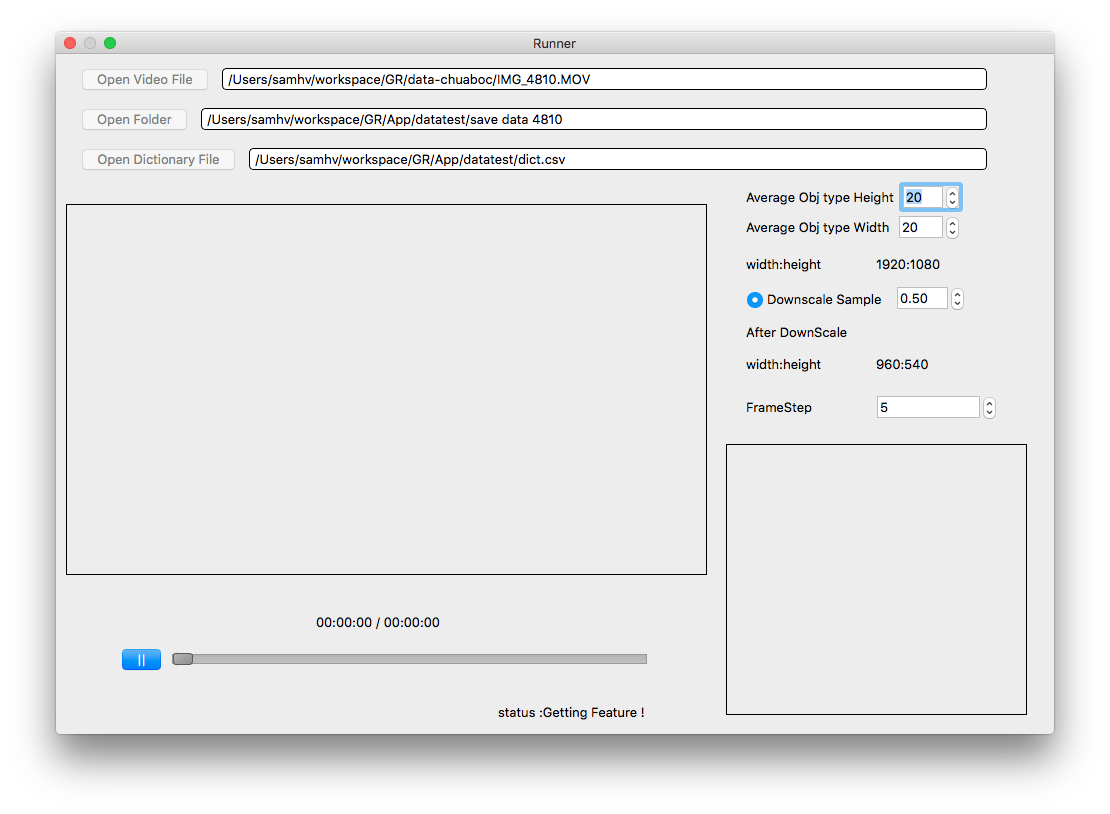
\includegraphics[width=\textwidth]{Chapters/Fig/Runner}
      \caption{Runner}
      \label{fig:Runner}
  \end{figure}
\end{center}
Fig \ref{fig:Runner} show the Runner, where client load the video and model for estimate the number of objects \\


\section{Implement}
This chapter shows details of Implementations of application. \\
\subsection{Application Architecture}

The Application is Implemented in $C++$ and QT framework with following module:\\
\textbf{Marker: }
\begin{itemize}
  \item \textbf{dialogmarker.ui} File that contains config for UI for dialog marker
  \item \textbf{dialogmarker.cpp} $C++$ source code that handle the UI signal and connect UI with \textbf{MarkingWorker}
  \item \textbf{dialogmarker.h} Header of diaglog that define UI
  \item \textbf{MarkingWorker.cpp} $C++$ source code of worker that use in UI for doing Job for UI, handle marking data
  \item \textbf{MarkingWorker.h} Header of worker that use in UI for doing Job for UI
\end{itemize}

\textbf{Trainer: }
\begin{itemize}
  \item \textbf{dialogtrain.ui} File that contains config for UI for dialog train
  \item \textbf{dialogtrain.cpp} $C++$ source code that handle the UI signal and connect UI with \textbf{TrainingWorker}
  \item \textbf{dialogtrain.h} Header of diaglog that define UI
  \item \textbf{TrainingWorker.cpp} $C++$ source code of worker that use in UI for doing Job for UI, where learning method integrated 
  \item \textbf{TrainingWorker.h} Header of worker that use in UI for doing Job for UI
  \item \textbf{ListModel.cpp} $C++$ source code of samples and object types models for table show in list view 
  \item \textbf{ListModel.h} Header of \textbf{ListModel.cpp}
\end{itemize}

\textbf{Runner: }
\begin{itemize}
  \item \textbf{dialogrun.ui} File that contains config for UI for dialog run
  \item \textbf{dialogrun.cpp} $C++$ source code that handle the UI signal and connect UI with \textbf{MarkingWorker}
  \item \textbf{dialogrun.h} Header of diaglog that define UI
  \item \textbf{RunningWorker.cpp} $C++$ source code of worker that use in UI for doing Job for UI, handle estimate of counting objects in video 
  \item \textbf{RunningWorker.h} Header of worker that use in UI for doing Job for UI
  \item \textbf{SampleDetail.cpp} $C++$ source code of Model data for table show in list view 
  \item \textbf{SampleDetail.h} Header of \textbf{SampleDetail.cpp}
\end{itemize}

\textbf{Not in Any module: }
\begin{itemize}
  \item \textbf{ObjectMark.cpp} $C++$ source code for store marker data 
  \item \textbf{ObjectMark.h} Header of \textbf{ObjectMark.cpp}
  \item \textbf{ViewerLabel.cpp} $C++$ source code For make label become viewer and clickable 
  \item \textbf{ViewerLabel.h} Header file of \textbf{ViewerLabel.cpp}
\end{itemize}


